\chapter{Introduction}
\label{chapter:introduction}
\section{Motivation}
Proteins are complex macro-molecules used by all living organisms in their biological processes and as such, proteins can be considered one of the building blocks of life. They are crucial to cell functions and so has widespread application to biological industries such as agriculture, food, medicine, cosmetics, as well as countless chemical products. Besides industrialism, the increased understanding of proteins and their complex behavior informs our perpetual development of better, more useful tools against human suffering and sickness. Protein function and properties lie at the heart of almost any biological process within us, and is thus a key to not just saving lives, but also their improvement. The synthesis of useful proteins is critical for these applications. However, finding useful proteins is a daunting task, especially when such proteins deviate significantly from those found in nature. The abundance of proteins makes laboratory experiments fall short at the scale at which proteins are discovered and stored. Other approaches are needed to adress this, and bioinformatics is the use of computational tools to aid the search and investigation of proteins.

Due to the extreme complexity of proteins, their analysis and optimization becomes difficult. In recent years, machine learning methods have been applied to a wide variety of problems with success in many fields. The successful application of machine learning on proteins could allow the discovery of new, useful proteins. Not only that, but an explosion in the amount of available raw protein data has happened in recent years, reaching hundreds of millions of protein sequences \cite{uniprot2007universal}. The disparity in raw sequences versus sequences with associated properties necessitates the use of learning methods, which solely analyze the raw sequence and does not rely on manual, human annotation. Such unsupervised methods would have to be tractable on a large dataset, and should ideally facilitate the exploration of new, useful proteins. For these requirements, representation learning seems fitting.

In the ideal case, representation learning enables the transformation from arbitrary protein sequences into compact representations, and vice versa, living in a smooth space. Such a learned representation should contain the essential features which describe a protein, and the discovery of new proteins should be feasible by exploring the smooth space, rather than exploring the space of proteins directly. Due to the complexity of proteins, such transformation onto proteins involves some degree of uncertainty. A probabilistic representation learning model would mitigate this by explicitly incorporating such uncertainty into the transformation by producing a distribution over representations. This distribution would inform the application of the representations and be of great use in settings where the degree of confidence in predictions are of consequence. A distribution over representations also affords sampling of representations, and so proteins can be generated from such models.

Unfortunately, such ideal representations are currently beyond the reach of modern representation learning methods. There are several issues that hinder the production of the above ideal representations. It is not obvious how a model is supposed to learn how to produce ``good'' representations that live in a smooth space (if a smooth space of protein representations is even sensible). Proteins are inherently sequential in nature -- how should a model reduce a protein sequence of arbitrary length into a fixed-size compact representation? Similarly, how should a model decode a representation back into a protein sequence, and how is it supposed to handle the inherent uncertainty that this involves? Considering the size of the entire (global) protein space, it may also be far too optimistic to represent all proteins in a compact representation space, and smaller, local regions of the protein space (protein families, for instance) may have to suffice, leading to smaller, less generally useful representation models.

The above issues raises several interesting fundamental questions, some of which  we would like to explore in this thesis:
\begin{itemize}
    \item To what extent do recent advances in protein deep learning reach such ideal representations as outlined above?
    % \item How can these be implemented in a modern machine learning framework?
    % \item What is a good protein representation?
    \item What are the advantages and disadvantages, if such exist, of global versus local representations?
    \item How does the choice of the representation affect the performance on select downstream tasks?
    % such as mutation effect prediction?
    % \item How does the properties of the representation affect the performance on a downstream task such as mutation effect prediction?
\end{itemize}

% Still, while no model can be said to have achieved the ideal, there are some avenues with varying amounts of success. Different models require different trade-offs. Predominant among these trade-offs is the choice of a global versus local representation -- that is, whether the model works with the entire protein space or just a subset. A model working on the global protein space necessitates a higher complexity and may be ineffective on the finer local scale. A model working on the local protein space only works with a certain region of the protein space, but this also leads to less complexity, and allows the use of sequence alignments, which we discuss in section \ref{sec:sequence_alignments}.

% Because proteins are sequential structures, concepts used in other sequential learning settings prove useful. For example, natural language processing (NLP) also deals with sequences with complex, long-ranged dependencies. One of the techniques used in NLP include recurrent neural networks (see section \ref{sec:recurrent_neural_networks}).

\section{Outline and delimitations}
This thesis is focused on applying representation learning to protein sequences. We examine the performance of different representations and their implications for protein informatics by developing three select models capable of working on protein sequences. Each model approaches the task in its own particular way and is chosen based on shown merits. All the models are trained to reconstruct their input, an unsupervised task. A key goal is, if possible, to systematically discern the design choices of the model architectures that yield superior performance on a chosen set of protein analysis tasks.%: mutation effect prediction.

Suitable background theory is provided before the models-, experiments- and discussion chapters. In chapter \ref{chapter:representation_learning}, the task of learning representations is introduced, providing a foundation for the notion of a ``good'' representation. Chapter \ref{chapter:probabilistic_modelling} on probabilistic modelling gives much of the background needed for the probabilistic model, the variational autoencoder, relying on approximation and inference. In a similar fashion, chapter \ref{chapter:sequence_learning} introduces sequence learning, which is the basis of the two remaining models. After these chapters, the reader should be ready to understand the concepts used to apply the model architectures. These are the focus of chapter \ref{chapter:models}. We start by presenting a single strictly local model, before presenting two different approaches to global models.

In section \ref{sec:unirep_model} we present UniRep \cite{alley2019unified}, a recurrent model. UniRep utilizes recurrent neural networks to process protein sequences, which allows it to function on the global protein space and has previously been shown to work well on this space \cite{alley2019unified}. %The output of the model can be transformed into a fixed-size representation, but it is unclear how to transform this representation back into a protein sequence.

In section \ref{sec:variational_autoencoder_model} we present a Variational Autoencoder (VAE), which uses protein sequences aligned to a fixed-length to allow the use of simple linear neural networks, and to take advantage of regularities that can be related to absolute positions within such an alignment. Since the VAE only works with aligned protein families, it is a strictly local protein model -- as such, the VAE will serve as the main local model in our comparison of local and global models. The VAE constructs a representation by encoding a protein sequence into a fixed-size, latent, probabilistic vector, which through a Bayesian neural network can be decoded back into a protein sequence.

Finally, in section \ref{sec:wavenet_model}, we present a convolutional model inspired by the WaveNet \cite{oord2016wavenet} architecture -- for lack of a better name, we will simply refer to this model as ``WaveNet'' in this thesis. WaveNet uses layers of causal convolutions, with progressively larger dilation to analyze the protein sequence. It can, in principle, process proteins of arbitrary length, allowing it to train on the global protein space, but as far as we are aware, this has not been attempted yet. It has however shown promise when trained on local protein families \cite{riesselman2019accelerating}. The model does not produce an explicit representation, but a representation may be obtained similarly to UniRep.

%Finally, in section \ref{sec:transformer_model}, we present the Transformer model \cite{vaswani2017attention}, a model based on the concept of ``attention'', which has been hugely successful within natural language processing. The model has desirable non-recurrent properties that allow for fast training, while maintaining variable-length input. However, like UniRep and WaveNet, it lacks an explicit representation.

These models represent different approaches to the protein representation learning problem. The VAE is a model restricted to aligned protein families (local), but this brings with it the advantage of lower complexity. The other models work with unaligned sequences (global) and are thus more general, but this also requires a more complex model, capable of finding patterns among variable-length sequences.

% \{inflate contribution :P write out details for each model, i.e. for VAE we showed that.. etc} 
% an examination of the relationship between global and local protein models and the effectiveness of various types of models on the protein representation learning task. This work required the development of the three models, all of which are largely inspired by contemporary research within the field.

To summarize, our contribution in this thesis initially includes an explanation and implementation of three conceptually different protein representations models. We subsequently provide comparable benchmark performances on benchmark protein analysis tasks suitable for evaluating the quality of the produced protein representations. In addition, we perform a detailed examination of the relationship between global and local protein models, providing a systematic foundation for representation selection. UniRep has previously been evaluated on general protein tasks with favor. We provide an extended investigation into its representations and their merits on local protein space. Likewise, WaveNet has been applied to local mutation effect prediction; we reproduce these experiments, and additionally provide protein representations directly extracted from this model. We measure and compare the performances of these representations with UniRep on general protein analysis tasks.

% \{general intro}
% thesis roadmap
% \begin{enumerate}
%     \item proteins are useful, complex and ubiquitous.
%     \item scalable statistical tools for analyzing the abundant proteins available ($\approx$220 milion) have become not only feasible, but also a potential source of discovery for the properties of proteins.
%     \item expert systems can transform raw protein sequence into efficient representations containing characteristic features. Such expert systems has become autonomous with deep learning.
%     \item this is desirable because it (potentially) yields a scalable, data-efficient process to capture useful protein features that can be used for downstream tasks in protein analysis. Some representations allow for exploration in protein space along properties of interest.
%     \item the data generating process, evolution of proteins, is so complex that any transformation of proteins into representations involves some degree of uncertainty. Probabilistic models explicitly incorporate such uncertainty into the process by producing distributions over representations. Not only does this allow the model to tell us "I do not know how to represent this protein", i.e. how much you should trust the representation, it also makes it possible to sample candidate representations.
%     \item because proteins are sequential (chains of amino-acids), concepts used in sequential learning and natural language processing also apply to the problem of learning protein representations from protein sequence. We look at some models that exploit this commonality.
%     \item different models requires different trade-offs: some models work on subsets of protein space by aligning proteins, others are functions over the entire domain of proteins.
%     \item we have explored 4 different models, that each capture at least one of the above modelling aspects (local/global protein input, aligned/unaligned proteins, latent models and recurrent models) and assessed their performance on predicting favorable attributes, mainly stability.
%     \item The first model is a variational autoencoder that is a latent space based model that is trained on reconstructing the input. In our settings, this is restricted to aligned, local protein input families.
%     \item A second model is UniRep, a recurrent, global, unaligned model that produces representations of proteins by taking the mean over its internal hidden representations. The advantage is the breadth of use.
%     \item A third model is a convolution-based model originally used for continuous sequential input (sound). This model performs comparably with the variational autoencoder, while removing the restriction to aligned protein data. The model lacks an explicit protein representation, but this can be potentially remedies in a fashion like UniRep.
%     \item Finally, we have applied an attention-based model (transformer), which have shown to be very performant in natural-language settings. This model has desirable non-recurrent properties that allow for fast training, while maintaining variable length input. It also allows for both local and global protein input. However, like the UniRep and WaveNet model, it lacks an explicit representation.
%     \item \{write a paragraph going along the lines of "To conclude, our contributions in this thesis are $\ldots$}
% \end{enumerate}

\section{Introduction to Proteins}
Proteins are large molecules (macromolecules) that are used by organisms in virtually every part of their function, such as enzymes or hormones. However, proteins are also widely used in the biological industries for a variety of purposes, including medical purposes, food processing and biological detergents. %These industries would benefit greatly from an increased understanding of proteins, as this would aid their efforts in protein engineering. Protein engineering is the process of developing and synthesizing useful proteins for the above-mentioned industries.

%\{refactor: wouter thinks its hverdagssprog}
%The central objects of study in this work are proteins. The complexity of proteins begs some explanation, which we provide here for the non-biologically oriented reader, who may not already be familiar with this topic.

%Aside from this background, we do not further significantly concern ourselves with the biological particularities -- we are computer scientists, not biologists. For the same reason, we apologize for any errors or shortcomings of the following explanation.

%\{define amino acid residue: basically when amino acids are chained together in a protein, the component of each amino acid that is not chained together is called the residue, i.e. the part that is left after making the protein.}

%\subsection{Function}

%\subsection{Construction?}
\subsection{Structure}
\label{sec:protein_structure}
Proteins consists of long chains of \textit{amino acids}. Amino acids are a class of organic compounds, of which about 20 different acids are used in proteins. Proteins commonly consists of hundreds of amino acids (sometimes referred to as \textit{residues}), connected together in a sequence, making proteins molecules of potentially thousands of atoms. In nature, proteins are constructed by organisms by reading their genetic code, in the form of DNA. The genetic code (genes) of the DNA describes which amino acids to put together in a sequence, in order to construct the desired protein. 

A protein is in theory defined entirely by its amino acid sequence. However, when proteins are assembled, the chain of amino acids folds up into a complex 3-dimensional structure. This structure is what largely determines the function and properties of the protein. When speaking of protein structure, we concern ourselves with three main levels of structure:

\begin{description}
    \item[Primary Structure:] Purely the 1-dimensional amino acid sequence itself, with no additional information about the 3-dimensional structure of the protein.
    \item[Secondary Structure:] 3-dimensional structure of local parts of the protein. When folding, local parts of the amino acid sequence arranges itself into certain structures, most commonly \textit{$\alpha$-helices} and \textit{$\beta$-sheets}. Secondary structure is knowing at each position of the protein, how the amino acid participates in local structure at that position.
    \item[Tertiary Structure:] The full specification of the folded protein, that is, the 3-dimensional coordinates of all the amino acids.
\end{description}

See figure \ref{fig:protein_structure} for an illustration of the three levels of protein structure.

\begin{figure}[ht]
    \centering
    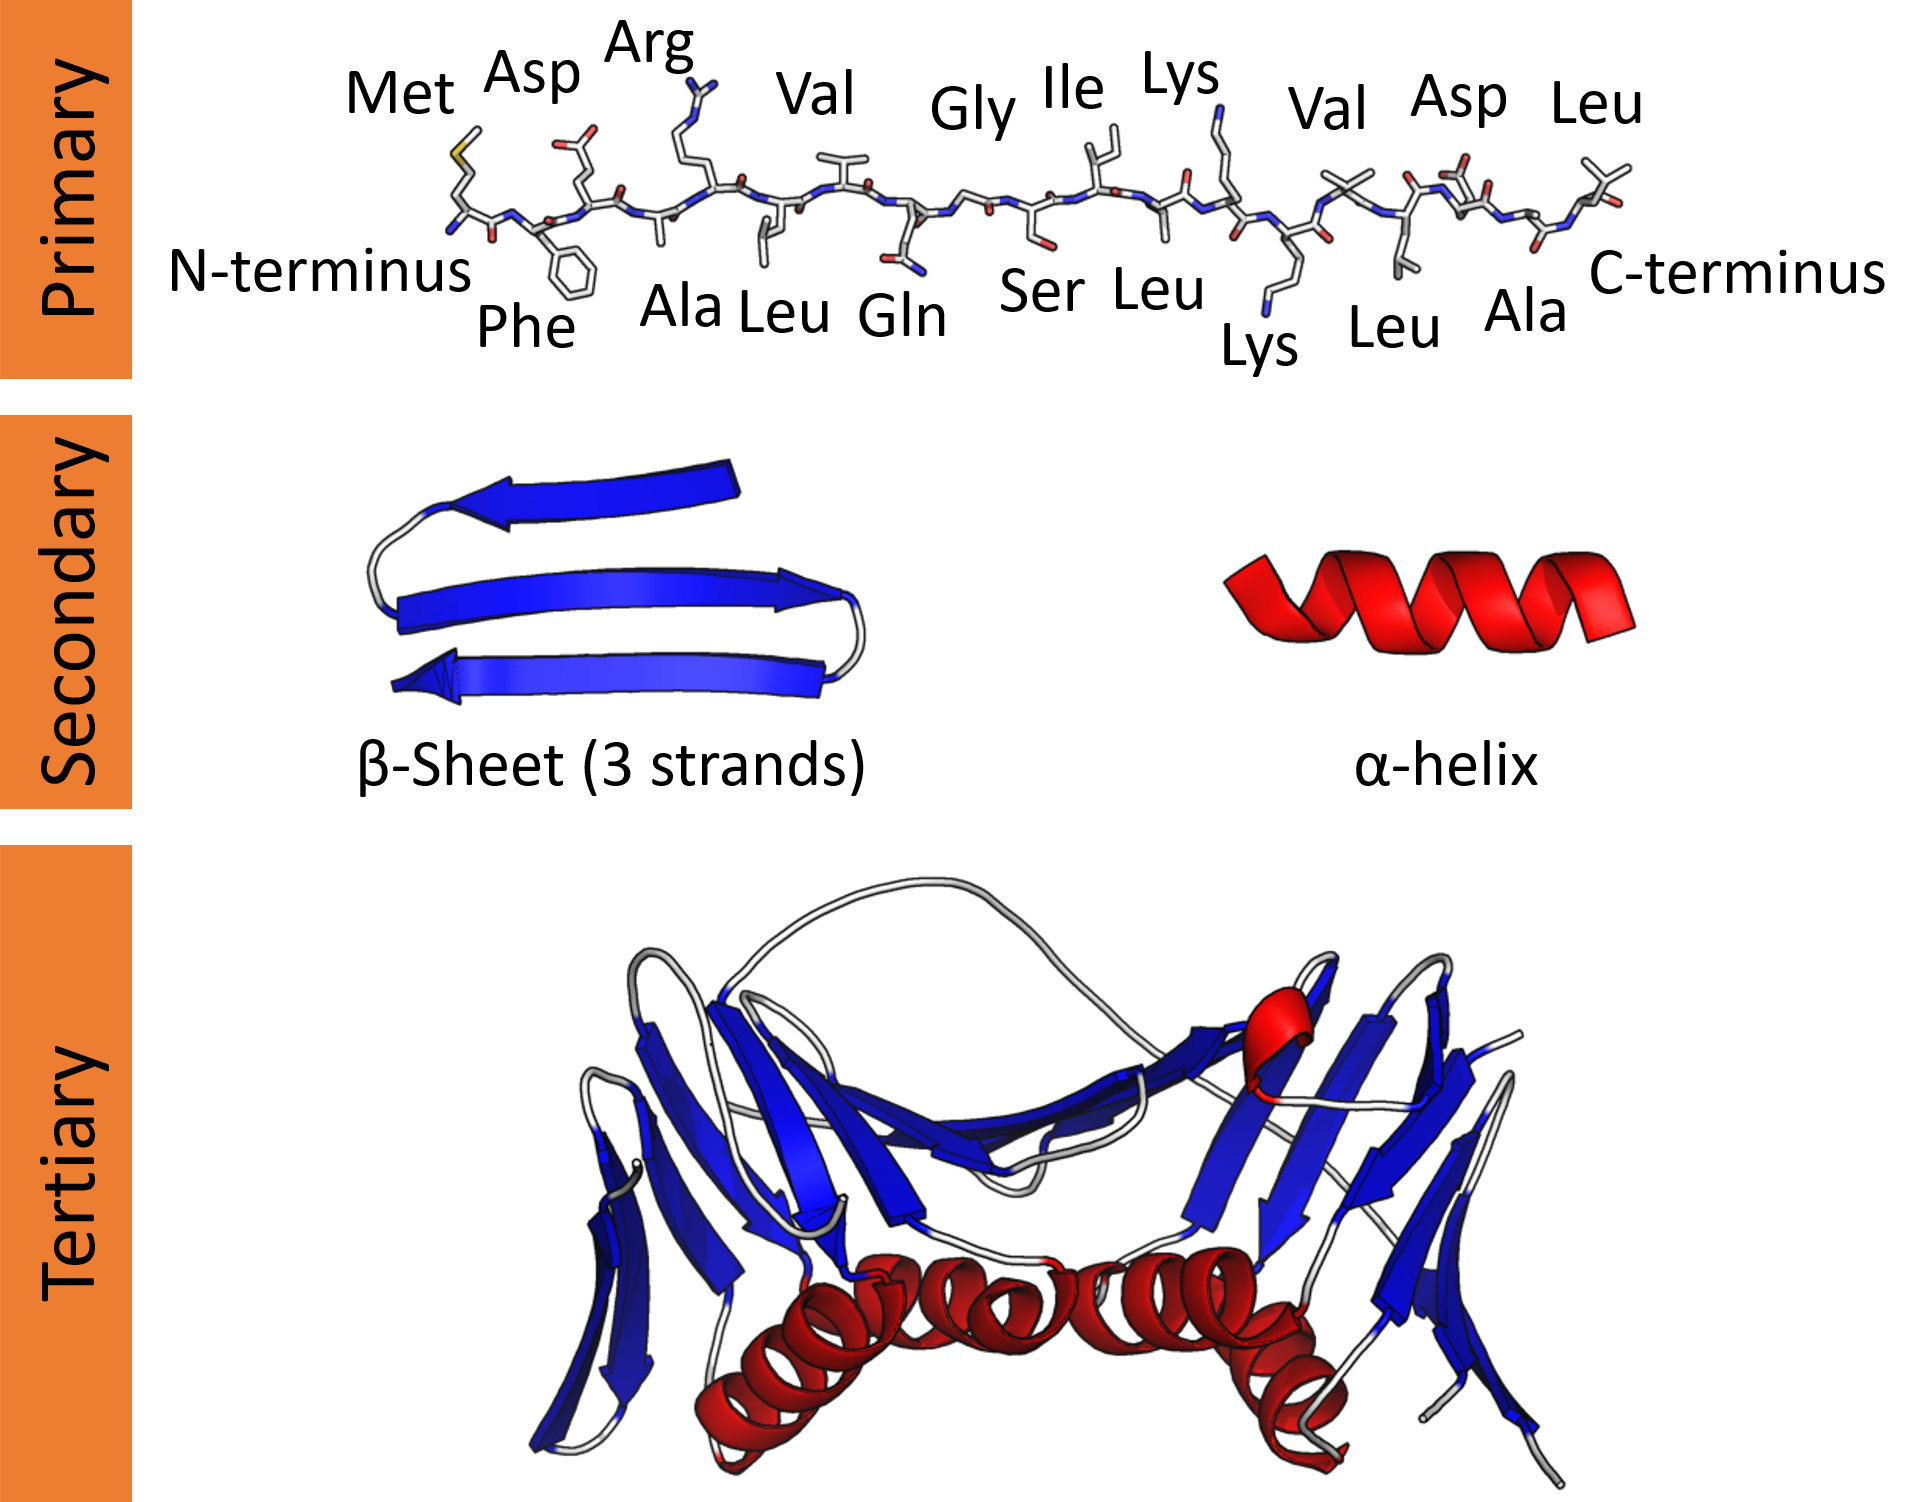
\includegraphics[width = 0.75\linewidth]{report/figures/protein_structure.png}
    \caption{Depiction of the levels of protein structure -- primary, secondary and tertiary. Note that the primary structure only consists of the sequence of amino acids, not any of the atoms' coordinates. Figure provided by \textcite{protein_structure_fig}.}
    \label{fig:protein_structure}
\end{figure}

A central task in protein machine learning is prediction of secondary or tertiary structure, given the primary structure. Many models have some success when predicting secondary structure, as it is not a very difficult task. Comparatively, predicting tertiary structure from primary structure alone is an incredibly difficult task, as the folding of a protein is such a complicated process.

%\{we only do the prediction as a validation, the representation from of primary sequence is the main concern. Refer to NLP language models}

In this work, we concern ourselves with useful representations derived from the primary structure alone. In doing this, we consider the protein's primary structure as merely a sequence of the common amino acids. Since there are not that many, each amino acid can be assigned a letter of the alphabet, resulting in a protein being represented as merely a string of letters (i.e., ``LDRSIEKFMK...''). This actually makes representation learning on proteins rather similar to representation learning on natural language, at least in its technical specification (to produce a representation given a list of tokens).

\subsection{Protein Families}
\label{sec:protein_families}
In addition to the structure of a single protein, proteins also partially share more abstract structure between them, due to their connected origins. This causes proteins to be clustered into what we call \textit{protein families}.

As organisms reproduce, their genetic material experiences random mutations -- these mutations in turn cause mutations in the organisms' proteins, which may change the proteins' function. Through the process of natural selection, the organisms which experience beneficial protein mutations continue reproducing, while organisms with detrimental protein mutations die out.

%Basically, just as evolution works on organisms as a whole, there is also evolution in proteins (really, one could say that the latter causes the former). 
Hence, just as different organisms are related in species or families, so are proteins related. This causes proteins to be structured in a phylogenetic tree, just as organisms are. We may use this information to our advantage to construct what is known as \textit{sequence alignments}, which we will discuss in section \ref{sec:sequence_alignments}.

\subsection{Methodological Relation to Natural Language Processing}
In natural language processing (NLP), most often data is in the form of written text, usually represented as a sequence of words. We can view our protein data as a similar sequence, except that the words of proteins are amino acids, and while natural languages has hundreds of thousands of words, proteins have just 20 amino acids. Proteins can be thousands of amino acids long, and similarly, documents may be thousands (if not tens or hundreds of thousands) of words long. It is clear that, despite some differences, representation learning in NLP and protein machine learning are related.

With this relation in mind, we look to NLP for inspiration for methods in machine learning to apply to proteins. As it turns out, many of the ideas in NLP can also be used in protein machine learning. In NLP there is the idea of a ``language model'', that is, a model which is able to predict (and hence produce) natural language following a given piece of text. This requires the model to learn the fundamentals of natural language, its interconnected dependencies and the probabilities of certain words following other words. Often a model will produce a representation of the text seen so far in order to inform the language generating process.

With proteins, a similar model would be very useful. Such a model could be trained to predict the following amino acids, given a part of a protein. As part of this training, it would have to learn a good representation of the protein in order to inform the generation of the amino acids. The hope is that such a model would have learned the fundamentals of the ``language of proteins''. %By validating on downstream tasks, such as predicting protein properties (like stability or the effect of mutations), one can assess whether the representation lives up to that hope.

\section{Related Work}
Machine learning has been an active research topic for some time. Protein machine learning has been a part of this development and many different approaches have been explored -- however, the results are not as dramatic as in some other machine learning fields, such as computer vision. Proteins seem to present a more substantial challenge for learning models, which is not too surprising given their complexity.

As computer scientists, we have had to familiarize ourselves with this research field. We have primarily studied fairly recent papers on novel model architectures that show promise on the protein representation learning problem.

In 2018, Riesselman, Shin, Kollasch et al. presented a Variational Autoencoder (VAE) architecture capable of encoding and decoding protein sequences \cite{riesselman2018deep}. The model was shown to perform well on predicting mutation effects, but also requires an aligned protein family. Our exploration of VAE's on proteins is largely inspired by their efforts and we use their aligned protein family datasets for training our models.

In 2019, Alley et al. presented the UniRep (``\textbf{Uni}fied \textbf{Rep}resentation'') model, which allows processing of variable-length proteins \cite{alley2019unified}. This enables training on the global protein space, after which a representation of a protein can be obtained from the model. The UniRep representation showed promising results on standard protein prediction metrics. However, the model does not include a decoder so the representation cannot be transformed back into a protein.

In 2019, Riesselman, Shin, Kollasch et al. proposed a new convolutional model \cite{riesselman2019accelerating}. It was inspired by the WaveNet architecture, a kind of causal convolutional neural network originally used for audio processing \cite{oord2016wavenet}. The model achieved similar performance to the VAE on local protein families. %Like UniRep, the model can produce a protein representation, but it lacks a decoder.

%\{Talk about the papers we have read related to this}

%\begin{itemize}
%    \item DeepSequence VAE \cite{riesselman2018deep}
%    \item UniRep paper: \cite{alley2019unified}
%    \item WaveNet paper: original \cite{oord2016wavenet} and DeepSequence %\cite{riesselman2019accelerating}
%\end{itemize}

% the problem (description)
% current state of the art - problems and status
% two problems: ...

% (1) no direct generative process, no interpolations with current methods (unirep)
% (2) it is not a probabilistic model; Uncertainty is not accounted for

% without a probabilistic model, the representation cannot actively be used as a

% our project

% why we chose to be two working on the project.

% Why is this interesting for NN and NZ:

% proteins based drugs.
% peptider mutationer

% This is fine for your MSc project. For the Novo grant, we will need to spice it up a bit, adding some comments about ultimately impact etc.

% The structure of such applications is typically in the form of:
% 1. What is the problem. E.g "Understanding how mutations in amino acid sequences affect protein structure and function is a central challenge in computational biology, ..."
% 2. What are the limitations/problems with current state-of-the-art solutions to this problem. E.g., "recently important progress has been made in this area using representation-learning techniques, which have... However, current approaches have extracted such representations, as the internal state of... This makes it difficult to incorporate notions of uncertainty, and other essential properties that we would normally impose on representations. ... In addition, current approaches are not generative, in the sense that we cannot generate protein sequences corresponding to any point in latent space. "
% 3. What will you do. "In this project, we will investigate the possibility of learning
% 4. How will this improve the world.

% \section*{Background}
% Understanding how mutations in amino acid sequences affect protein structure and function is a central challenge in computational biology. Machine learning has proven to be a useful tool in the analysis of protein sequences. One form of machine learning that has been effectively applied to this problem is \textbf{representation learning}.

% Representation learning is the task of training a machine to produce a suitable representation of features for the desired input, as opposed to manually engineering the representation. Good representations are important in order to learn useful properties of the given data.

% Previous attempts at \textbf{protein sequence learning} have shown that fundamental structural features, that capture the function of a given protein, can be learned and represented from raw protein sequences by using Deep learning \cite{alley2019unified}. Specifically, using a \textbf{recurrent neural network} to summarize any protein sequence into a fixed length vector and subsequently averaging, such statistical representations can be discerned from large sets of input data. Additionally, such approaches have been shown to improve performance in nearly all models on downstream tasks \cite{rao2019evaluating}.

% Protein sequences are \textbf{comparable to natural language sentences}: both consists of a sequence of symbols. Sentences consists of the letters of the alphabet, while proteins are amino acids. Thus one might look at the results of natural language sentence representations in order to learn about protein sequence representation. A study by Google Brain \cite{bowman2015generating} showed that one can represent entire sentences as single vectors in a \textbf{latent space}, allowing interpolation between sentences. Additionally, the latent space inherently maps common properties of sentences, such as style and topic. It is possible that a similar representation for proteins may be able to \textbf{map properties of proteins, such as secondary structure}.

% \textbf{Unsupervised learning} is particularly suited for protein machine learning, since there is an overweight of unlabeled data. If a powerful unsupervised model could be produced, the wealth of this data could be used effectively \cite{AlQuraishiUnsupervised}. Therefore, unsupervised or variants like semi- or self-supervised learning methods could be useful.

% Unsupervised representation learning has recently been applied to protein sequences \cite{alley2019unified} in order to achieve a latent space representation. However, current approaches have extracted such representations, as the hidden internal state of a recurrent layer in the learning network. This makes it difficult to incorporate notions of uncertainty, and other essential properties that we would normally impose on such representations. That is, current approaches are not generative, and so we cannot generate protein sequences corresponding to any point in latent space.

% Current work on representations of proteins might carry potential toward a \textbf{general representation of proteins}, implying that general unseen protein sequences can be analyzed with such a representation with respect to functionality or structure, or at least infer commonalities from their representations. We wish to explore such implications.

% \section*{Aims and Method}
% This project revolves around applying representation learning to protein sequences. We wish to examine the performance of representations and their implications for protein informatics, by developing an unsupervised representation of protein sequences, using tools from machine learning such as variational autoencoders and deep neural networks. The results will be compared with current state-of-the-art.

% Initially, we wish to inspect the unsupervised UniRep model \cite{alley2019unified} which compresses protein sequences into a fixed length vector, representing the sequence in a latent space. One key aspect is that the representations created by UniRep corresponds to the internal state of the LSTM used for training. In this project, we wish to make a proper representation instead, meaning that the representation itself is the output, not the internal state. The hope is that such a model would produce an overall better representation, with better performance on standard benchmarks.

% The latent space defined by such a representation might allow for an understanding of protein sequences, by defining a mapping from sequences to protein properties, such that similar proteins are close together in the space (see figure \ref{fig:latentSpace}). Previously unseen points could correspond to unseen protein sequences, and properties of these proteins could be inferred from the latent space.

% In addition, it will be useful to use representations to explain the behavior of variants of protein that we know, but we need to optimize. For example, the representation is important to help explaining the experimental results of variants screening, trying to map the effect of mutations, especially in case when we do not have a structure.

% \begin{figure}[ht]
%     \centering
%     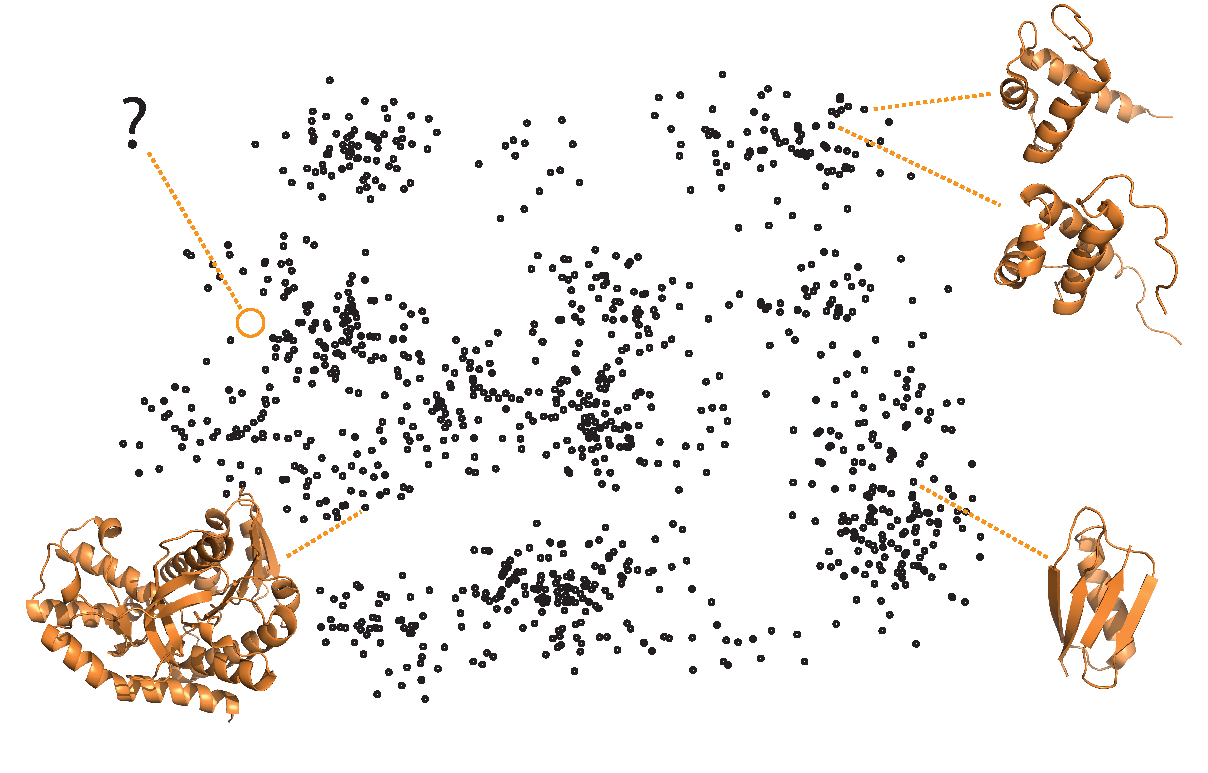
\includegraphics[width=\textwidth]{figures/figure.pdf}
%     \caption{A 2-dimensional view of a protein sequence representation. Similar proteins have representations that are close together. With such a representation, small changes in protein can be explored in the space by looking at points close to the protein. Properties of unknown sequences (represented here by the question mark) could potentially be explored by examining the representation space.}
%     \label{fig:latentSpace}
% \end{figure}

% \section*{Project Plan}
% We will start by identifying strengths and weaknesses in current state-of-the-art techniques. This would give us a solid foundation on which to build our new model.

% We wish to examine which types of neural networks best suit the learning task, by exploring both convolutional neural networks (CNNs) and recurrent neural networks (RNNs).

% Then we assess the quality of different types of representations, such as those achieved by considering the entire sequence at once versus representations as a combination of sub-representations of the sequence's components.

% Finally, to evaluate the project aims, we will compare the results with the current state-of-the-art. Table \ref{schedule} shows a proposed schedule for the project.

% \begin{center}
% \begin{table}[H]
% \begin{tabular}{lclll}
% \textbf{Project Plan} & \textbf{Schedule (months)}        &  &  &  \\ \cline{1-2}
% \multicolumn{1}{|l|}{\begin{tabular}[c]{@{}l@{}}Preliminaries: \\ Identify strengths and weaknesses on current state-of-the-art\end{tabular}}                         & \multicolumn{1}{c|}{1}   &  &  &  \\ \cline{1-2}
% \multicolumn{1}{|l|}{\begin{tabular}[c]{@{}l@{}}Modelling: \\ Recurrent vs Convolutional Neural Networks\end{tabular}}                                                     & \multicolumn{1}{c|}{1-3} &  &  &  \\ \cline{1-2}
% \multicolumn{1}{|l|}{\begin{tabular}[c]{@{}l@{}}Latent space structuring: \\ Entire sequence representation vs. position representation and transitions\end{tabular}} & \multicolumn{1}{c|}{3-5} &  &  &  \\ \cline{1-2}
% \multicolumn{1}{|l|}{\begin{tabular}[c]{@{}l@{}}Applications: \\ Performance of results in comparison with current-state-of-the-art\end{tabular}}                     & \multicolumn{1}{c|}{6}   &  &  &  \\ \cline{1-2}
% \end{tabular}
% \end{table}
% \label{schedule}
% \end{center}

% \section*{Feasibility}
% This project is ambitious, but we both have strong backgrounds in computer science, with bachelor degrees with very high average grades. We finished our bachelor degrees with a project within the field of machine learning as well, and wish to repeat the success. During our master's degree we have taken multiple elective courses in machine learning, which will be invaluable to this project.

% We chose to work as a group because of two factors: the project scope and its length. While the project is ambitious, we only have 6 months to complete it. A single student would likely not be able to achieve this. Please note that because of the duration of the project, funding both of us through the scholarship amounts to the same expense as supporting a single student for a longer project of 12 months, which is common in other university departments.

% The project will be supervised by Wouter Krogh Boomsma, who specializes in machine learning methods for biomolecular data at the Department of Computer Science, University of Copenhagen, which provides an ideal setting for the execution of this project.

% Wouter has existing collaborations to Novozymes (Lars Olsen, Protein Engineering), on the task of protein stability prediction. One of the ideas behind the current MSc project was to establish closer ties to protein research at Novo Nordisk, through this collaboration with Research Scientist Daniele Granata, in the Modelling and Predictive Technologies Department.

% \section*{Interest to Novo Nordisk and Novozymes}
% The application of protein sequence representations could be immense within analysis and understanding of new proteins and their function, especially when detailed structural information is not easily available. Importantly, the approach will give the opportunity to build tailored sequence models for specific classes of compounds of interest for Novo Nordisk and Novozymes, for example antibodies, nanobodies, or peptides libraries.

% Obtaining an accurate representation of protein sequences can represent a fundamental tool for interpreting and rationalizing the results of experimental screenings, enabling also the exploitation of other machine learning approaches toward the automatized generation of new variants.

% These ideas greatly agree with the recent efforts of Novo Nordisk to enlarge the exploitation of Data Science and AI technologies in its drug discovery process. We have no doubt that Novozymes could benefit from this technology as well.

% In addition, this field of research, being the understanding and formulation of protein sequence space, is comparatively new, allowing for many different ventures to be explored. This project is one step in that direction.

% I suggest that the goal of the main project should be that we try to create a proper representation, rather than simply using the internal state of the LSTM. We will do this by using variational auto encoders. The challenge here is that we need to encode *sequences* of inputs.

% Daniele
% Protein sequence models would be a great subject actually. Regarding the application, it seems pretty simple and it requires very little information in general and also for the project (Description of project in English, maximum 1,200 words. Please include background, aim and project plan and how this project is of interest to Novo Nordisk) especially if you have already proposals around.

% Wouter
% Unified rational protein engineering with sequence-only deep representation learning
% This is the first (or one of the first) applications of using language models to learn representations of protein sequences.
% https://www.biorxiv.org/content/10.1101/589333v1
% One of the authors, Mohammed Alquraishi (a collaborator of ours), also writes some of his thoughts on the method on his blog: https://moalquraishi.wordpress.com/2019/04/01/the-future-of-protein-science-will-not-be-supervised

% Evaluating Protein Transfer Learning with TAPE
% This is a very recent manuscript (will probably be published at NeurIPS this year) about representation learning of biological sequences. It is interesting because it asks the question how much different downstream tasks can be improved by first learning a good representation - and they present a benchmark set that is likely to become standard in the field (which we might use in the project).

% In the preproject, I suggest we try and reproduce the results of the first article, but with CNNs instead of RNNs. I suggest that the goal of the main project should be that we try to create a proper representation, rather than simply using the internal state of the LSTM. We will do this by using variational auto encoders. The challenge here is that we need to encode *sequences* of inputs. Here is one of the first papers that tries to do encode/decode sequences of words: https://arxiv.org/abs/1511.06349. There are a some difficulties getting this to work, and some newer references that try to resolve this, but I think you have enough reading material for now :) Again, we will try to use CNNs in addition to LSTMs, to compare pros/cons of the two approaches.

% I do not expect you to have a full overview over this literature when we meet - so don’t stress too much if there are things you don’t understand in these papers. But it would be great if you could try to write the main points of your thesis project in your own words - so we have something to discuss when we meet on the 27th.
